\subsection{}
All data was collected from runs on a Hamilton par7.q node.

Figure [Fig.\ref{fig:scaling}] shows the scaling characteristics of step 4 in terms of the number of bodies. 
We see from [Fig.\ref{fig:scaling_sub}] that scenarios with over 1000 bodies scale well to Hamilton's 24 cores, whereas models using $<$1000 bodies scale less well. 
If we assume this is a strong scaling model, following $t(p) = f \cdot t(1) + (1-f)\cdot \frac{t(1)}{p}$, we can calculate constant $f$ for each data point [Fig.\ref{fig:scaling_f}]. We can see scenarios with $>=500$ bodies are modeled well by the strong scaling model as there is a low variance of $f$ estimations, giving evidence that $f$ is a constant. 
However, the strong scaling model breaks down under $500$ bodies as $f$ is likely not constant. 
I suspect this breakdown is caused by the overhead for OMP to create and synchronize threads. 
This overhead is likely a function of the number of threads and could explain the speedup then slowdown for $200$ bodies.
We also see that $f$ decreases with more bodies. In my implementation some of the calculations with runtime $O(n)$ are done in series (where $n$ is number of bodies); However, all calculations with runtime $O(n^2)$ are done in parallel. Hence we would expect f to decrease as $O(n^2)$ dominates.

\subsection{}
The EM algorithm iterativley improves a model to fit a sequence of observed states. For a model $\lambda$ and observed sequence $x$ we seek to maximise $p(x|\lambda)$. Model $\lambda = (\pi, m, e)$ where: $\pi$ are the initial probabilities, $m$ are the transition probabilities, and $e$ are the emission probabilities.

To calculate $\hat{\lambda}$ we can use some helper functions. $\alpha$ is the forward algorithm.
\begin{gather}
    \alpha_1(i) = \pi_i e_i(O_1)\\
    \alpha_{t+1}(i) = e_j(O_{t+1}) \cdot \sum_{i=1}^N\alpha_t(i)m_{ij} \\
\end{gather}

$\beta$ is the backward algorithm
\begin{gather}
    \beta_T(i)=1\\
    \beta_t(i)=\sum_{j=1}^N m_{ij} e_j(O_{t+1}) \beta_{t+1}(j)\\
\end{gather}

$\gamma$ is the probability of being in a state given that we know the hole sequence.
\begin{gather}
    \gamma_t(i) = \frac{\alpha_t(i) \beta_t(i)}{\sum_{j=1}^N \alpha_t(j) \beta_t(j)}\\
\end{gather}

$\xi$ is the probability of transitioning from state i to state j given we know the entire sequence.
\begin{gather}
    \xi_t(i, j) = \frac{\alpha_t(i) m_{ij} e_j(O_{t+1}) \beta_{t+1}(j)}{\sum_{i=1}^N \sum_{j=1}^N \alpha_t(i) m_{ij} e_j(O_{t+1}) \beta_{t+1}(j)} \\ 
\end{gather}

Using these helper functions we can calculate the new components of $\hat{\lambda}$.
\begin{gather}
    \hat{\pi}_i = \gamma_1(i)\biggbreak
    \hat{m}_{ij} = \frac{\sum_{t=1}^{T-1} \xi_t(i,j)}{\sum_{t=1}^{T-1} \gamma_t(i)}\biggbreak
    \hat{e}_i(k) \frac{\sum_{\forall t: O_t = k} \gamma_t(i)}{\sum_{t=1}^T \gamma_t(i)}
\end{gather}

Iterating this process ($\lambda \gets \hat{\lambda}$) will converge on a local maximum for $p(x|\lambda)$.

We can tackle verification of the algorithm with 2 methods: testing helper function, observing expectation maximization. I verified each helper function with unit tests that: verify base cases (if applicable); and verify against known mathmatical identities, primarilly $\sum_{a \in A} p(a) = 1$. The following identites are tested. All free imply that the identiy hold over the indiciees domain, in some cases I test across the whole domain, in others just a sample, depending on what is computationally feasible.

\begin{gather}
    \sum_i \alpha_t(i) = 1 \\
    \sum_{x \in \Sigma^*} \beta_0(i) = 1\\
    \sum_{i} \gamma_t{i} = 1\\
    \sum_{i}\sum_{j} \xi_t(i, j)=1\\
    \sum_{j} \xi_t(i,j) = \gamma_t(i)\\
    \sum_i \hat{\pi}_i = 1\\
    \sum_j \hat{m}_ij = 1\\
    \sum_k \hat{e}_i = 1 \\
\end{gather}

Also we can see that for a an example sequence with a series of random seeds eexpeectation is maximised to seeveeral siffrent local minima. \cite{em}
\begin{figure}[h!]
    \begin{center}
    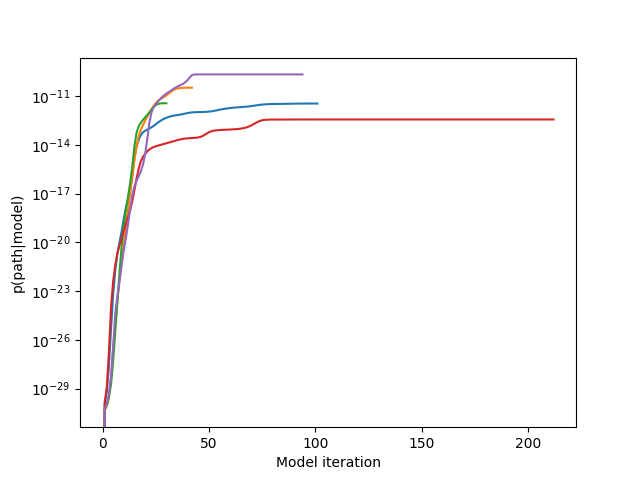
\includegraphics[scale=0.6]{EM.png}
      \caption{step 1 (blue) step 3 (orange). Change in errors for a 2 body system under extreme conditions (near collision).}
      \label{fig:convergence}
    \end{center}
    \end{figure}
